\newgeometry{margin=85pt}
\chapter*{Análisis espacial} \label{cap:analisis}
\setcounter{chapter}{4} 
\setcounter{section}{0}
\addcontentsline{toc}{chapter}{Análisis espacial}
El análisis espacial es la funcionalidad que caracteriza a los GIS. Consiste en manipular información espacial para extraer información nueva y significativa a partir de los datos originales. 

\section{Estadística espacial}
La estadística espacial es la reunión de un conjunto de metodología para el análisis de datos espaciales.
Estos datos corresponden a valores que toma una variable aleatoria en distintos puntos de una región. 
De manera más formal, se puede decir que la estadística espacial trata con el análisis de realizaciones de un proceso estocástico.
El proceso estocástico parte de la idea de que datos cercanos en espacio están presumiblemente correlacionados, 
recogida en las leyes de Tobler en el artículo \cite{Tobler1970}, concretamente en la denominada “Primera Ley de la Geografía” o principio de autocorrelación espacial, por la que:
“Todas las cosas están relacionadas entre sí, pero las cosas más próximas tienen una relación mayor que las distantes”.

A partir de esta noción, podemos definir un proceso estocástico como una colección de variables aleatorias \{{$Z(s) \in D$} / {$s \in R^d$}\},
en donde \textit{s} representa una ubicación que toma valores en el espacio $R^d$ d-dimensional 
y {$Z(s)$} es una variable aleatoria en la ubicación \textit{s} que toman valores en el espacio de estados $D \subset R^d$.
Si \textit{d} es igual a 2, $Z(s)$ puede asociarse a una variable medida en un punto \textit{s} del plano.
En términos prácticos, $Z(s)$ puede verse como una medición de una variable aleatoria, por ejemplo, la temperatura
en un punto \textit{s} de una región de estudio, representado por sus coordenadas geográficas o cartesianas.

Según esta definición, podemos interpretar a un proceso estocástico como una sucesión de variables aleatorias cuyas características pueden variar a lo largo del espacio. 
Pero también se puede definir un proceso estocástico en el que las variables aleatorias varían een función del tiempo.

El tipo de dato espacial a analizar permite una primera división de esta rama de la estadística.
Hablaremos de datos geoestadísticos si las ubicaciones \textit{s} provienen de un conjunto \textit{D} fijo y continuo, es decir, el área de estudio
está previamente delimitado por el analista, el cual toma puntos de observación en dicha región y en ellos mide alguna variable de interés.
Por otro lado, hablaremos de análisis de patrones espaciales si las ubicaciones \textit{s} pertenecen a un conjunto \textit{D} aleatorio, discreto o continuo, 
que no depende del analista.

\subsection{Análisis de patrones de puntos}
Uno de los objetivos principales del análisis espacial es la detección de patrones.
La disposiciones de los datos espaciales forman patrones de puntos, que permiten conocer el tipo de distribución que presenta una variable espacial en el espacio estudiado.

\subsubsection{Tipos de patrones}
\begin{figure}[H]
    \centering
    \subfigure[Agregado]{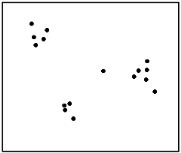
\includegraphics[width=0.25\columnwidth]{Imagenes/analisis/agregado.png}}
    \subfigure[Aleatorio]{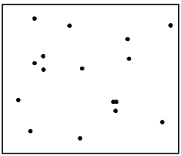
\includegraphics[width=0.25\columnwidth]{Imagenes/analisis/aleatorio.png}}
    \subfigure[Regular]{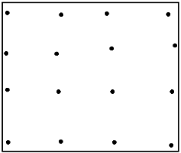
\includegraphics[width=0.25\columnwidth]{Imagenes/analisis/regular.png}}
    \caption{Tipos de patrones de puntos} \label{fig:patrones} 
\end{figure} 
\begin{itemize}
    \item Agregado: Los puntos se disponen formando grupos, por lo que la densidad es mayor en esas zonas. Un ejemplo de patrón de puntos agrupado son los casos de enfermedades infecciosas.
    \item Aleatorio: Los puntos no presentan una estructura claramente definida, sino que están distribuidos aleatoriamente a lo largo de todo el espacio.
    Un ejemplo son la localización de accidentes de tráfico en una ciudad.
    \item Regular: Los puntos se disponen alejados entre sí a una distancia semejante, por lo que la densidad es constante. 
    Un ejemplo son la posición de los paneles solares dentro de un parque fotovoltaico. 
\end{itemize}

\subsubsection{Medidas para determinar la distribución de los puntos}
Existen una serie de medidas para determinar la distribución de los puntos sobre el espacio:
\begin{itemize}
    \item Medidas que permiten calcular la densidad de puntos, número de puntos por unidad de superficie.
    \item Medidas que buscan determinar el carácter agregado, distribuido o aleatorio de los puntos sobre el espacio.
    Aquí se incluye la autocorrelación espacial, que mide el grado de agrupamiento o dispersión de los puntos, basándose tanto en las ubicaciones como en los valores que toman.
    Dado un conjunto de puntos y un atributo asociado a ellos, se emplea el Índice de Moran para evaluar si el patrón expresado está agrupado, disperso o es aleatorio. 
    \begin{figure}[H]
        \centering
        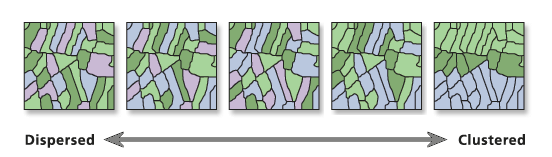
\includegraphics[width=0.85\textwidth, height=0.15\textheight]{Imagenes/analisis/moran.png}
        \caption{Transición de patrón disperso a agrupado} \label{fig:disperso_agrupado}
    \end{figure}
    El Índice de Moran es positivo cuando se agrupan los valores similares y negativo cuando se agrupan los valores disímiles. 
    En el caso de la figura \ref{fig:disperso_agrupado}, el Índice de Moran comienza con valores negativo para la imagen de la izquierda (patrón disperso) 
    y va aumentando su valor hasta llegar a la imagen de la derecha (patrón agrupado) con valores positivos. 
    \item Medidas centrográficas \\
    Las medidas centrográficas representan descriptores básicos de los datos espaciales, extendiendo las medidas de tendencia central,
    como la media o la mediana, y de dispersión, como la desviación típica, de la estadística clásica al ámbito espacial.

    \begin{itemize}
        \item Centro medio \\
        La principal medida de centralidad es el centro medio y se calcula como el valor medio en cada eje de coordenadas de los puntos analizados.
        Para un sistema bidimensional con un total de \textit{N} puntos, el centro medio es el punto $(\overline{x}, \overline{y})$ tal que:

        \begin{eqnarray}
            \overline{x} = \frac{\displaystyle \sum_{i=1}^n x_i}{N} \hspace{2em} \overline{y}= \frac{\displaystyle \sum_{i=1}^n y_i}{N} \nonumber
        \end{eqnarray}

        Podemos ponderar los puntos analizados según el valor \textit{a} de alguno de sus atributos, tal que:
        \begin{eqnarray}
            \overline{x} = \frac{\displaystyle\sum_{i=1}^N a_i x_i}{\displaystyle\sum_{i=1}^N a_i} \hspace{2em} \overline{y} = \frac{\displaystyle\sum_{i=1}^N a_i y_i}{\displaystyle\sum_{i=1}^N a_i} \nonumber
        \end{eqnarray}

        \begin{figure}[H]
            \centering
            \captionsetup[subfigure]{labelformat=empty}
            \subfigure{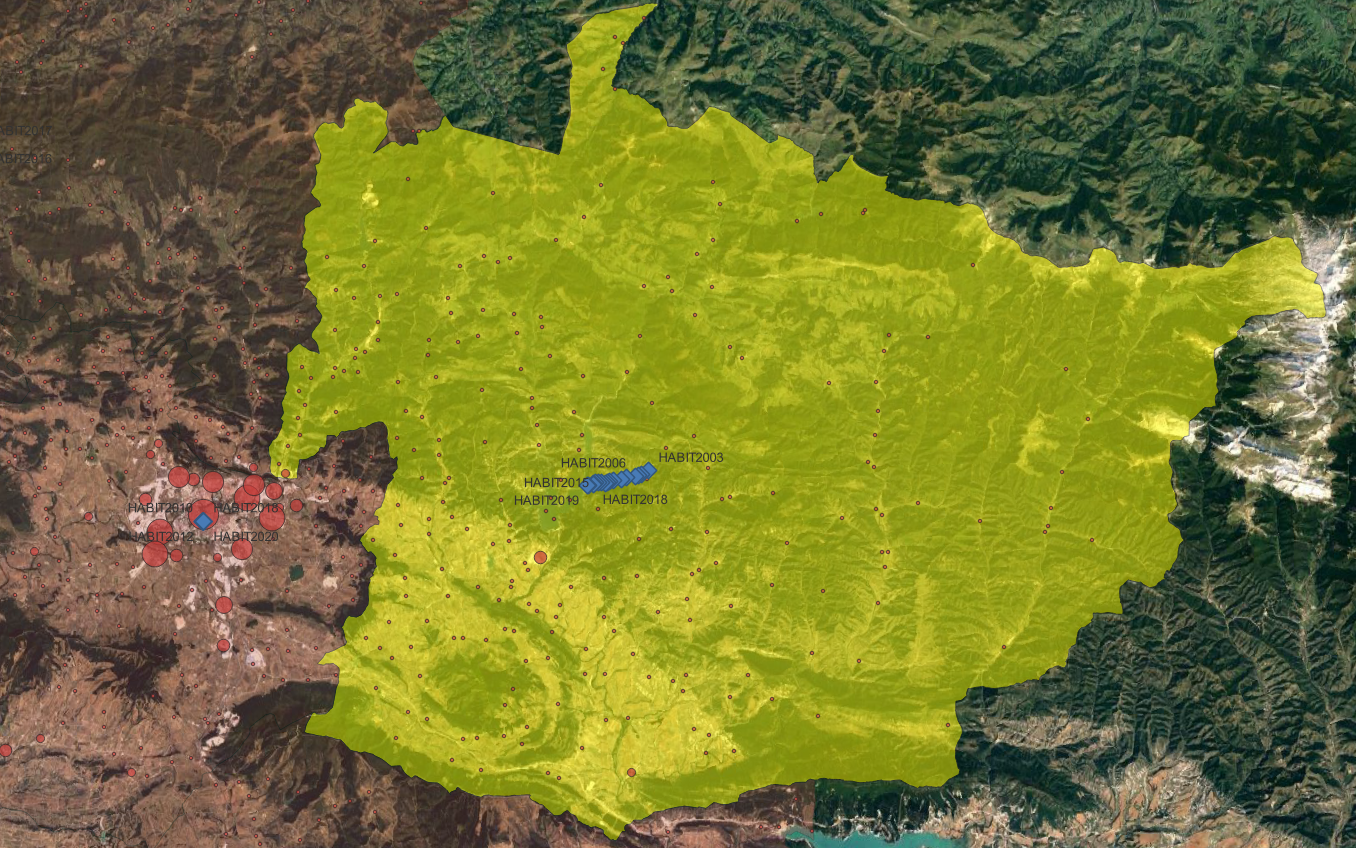
\includegraphics[width=0.65\textwidth, height=0.35\textheight]{Imagenes/analisis/centros-medios.png}}
            \subfigure{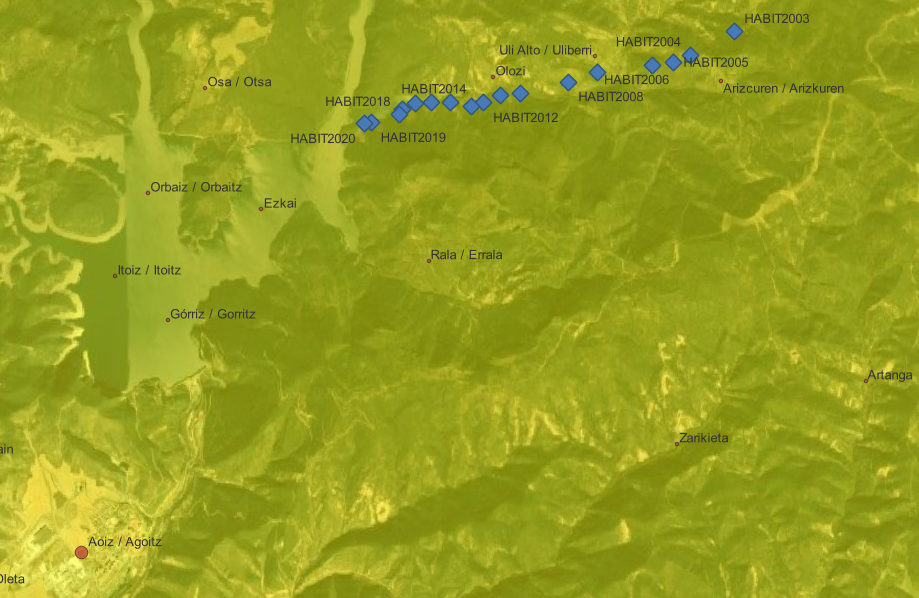
\includegraphics[width=0.65\textwidth, height=0.35\textheight]{Imagenes/analisis/centros-medios-zoom.png}}
            \caption{Centros medios demográficos en la zona del pirineo navarro} \label{fig:centros-medios} 
        \end{figure} 

        Un uso habitual del centro medio lo encontramos en los estudios demográficos.
        En la figura \ref{fig:centros-medios} podemos ver la evolución de las poblaciones sobre la zona del pirineo navarro y cómo se ha desplazado su centro medio a través del tiempo.
        Se puede apreciar una tendencia hacia zonas más pobladas como la capital (Pamplona) o el municipio con mayor población de la zona (Aoiz).

        \item Centro mediano \\
        El equivalente espacial de la mediana es el centro mediano, que se calcula como el valor de las medianas en cada eje de coordenadas de los puntos analizados.
        Resulta interesante trazar líneas de división que dividen el conjunto de puntos en dos partes iguales.
        Por ejemplo, en el ámbito demográfico, podemos dividir el territorio en dos zonas igualmente pobladas.

        \item Distancia típica \\
        En cuanto a las medidas de dispersión, el equivalente a la desviación típica es la denominada distancia típica, que se calcula como:

        \begin{equation} s_d = \sqrt{\frac{\displaystyle\sum_{i=1}^n d^2_i}{n}} \nonumber \end{equation}

        siendo $d_i$ la distancia entre el punto i-ésimo y el centro medio. 
        Se suele emplear la distancia euclidiana, tal que:
        \begin{equation}
            d_i = \sqrt{(x_i-\overline{x})² + (y_i-\overline{y})²} \nonumber
        \end{equation}

        Al igual que el centro medio, también podemos ponderar los puntos analizados según el valor \textit{a} de alguno de sus atributos, tal que:

        \begin{equation} s_d = \sqrt{\frac{\displaystyle\sum_{i=1}^n a_i d_i^2}{\displaystyle\sum_{i=1}^N a_i}} \nonumber \end{equation}

        Una forma de representar esta distancia típica es mediante un circulo de radio dicha distancia centrado en el centro medio.
    \end{itemize}
\end{itemize}

\subsubsection{Medidas para determinar la variación en el espacio}
Las medidas vistas hasta ahora definen la distribución en un espacio reducido, 
pero si queremos estimar el comportamiento de la variable espacial a lo largo de todo el espacio, 
entran en juego dos conceptos estadísticos: estacionariedad e isotropía.
Matemáticamente, decimos que un proceso es estacionario cuando no varía al transformarlo dentro de un espacio d-dimensional, e isotrópico cuando no varía por la rotación del punto de origen.
En el ámbito geográfico, la estacionariedad indica que las medidas centrográficas no varían con la traslación, es decir, 
que la función de distribución de probabilidad, la cual nos proporciona la probabilidad de que una variable tome cierto valor, es constante en el espacio.
La isotropía indica que las medidas centrográficas no varían con la rotación. 
Estas propiedades muestran el principio de replicación de un conjunto de datos. 
Por ejemplo, dos valores de una variable espacial con un comportamiento isotrópico y estacionario, separados por la misma distancia, deberán tener las mismas propiedades.

\subsection{Geoestadística}
La Geoestadística es un área de la estadística espacial que abarca al conjunto de técnicas usadas para analizar fenómenos que ocurren en la superficie terrestre y 
para predecir la distribución espacial de variables asociadas a dichos fenómenos.
Algunos ejemplos de estos fenómenos espaciales son la Meteorología, Epidemiología, Geomárketing o análisis geográfico de mercados, Demografía, Criminología, entre muchos otros.

La Geoestadística permite reducir los costes de recolección de datos espaciales, que dependiendo del sector en el que se aplique, pueden ser muy elevados.
Por ejemplo, en su origen (mediados del siglo XX), la Geoestadística se aplicó en la industria minera y de hidrocarburos,
generando modelos probabilísticos para predecir localizaciones de yacimientos potenciales.

\subsubsection{Interpolación}
La interpolación espacial es uno de los principales análisis geoestadísticos basado en la estimación de valores desconocidos de una variable espacial a partir de puntos con valores conocidos. 
Analiza y simula el comportamiento de los datos en un espacio muestral, así como su influencia en otros puntos cercanos.

En un GIS, la interpolación de esos puntos puede ser aplicada para crear una superficie ráster con estimaciones realizadas para todas las celdas del ráster.
Existen muchos métodos de interpolación, algunos de ellos son los siguientes:

\begin{itemize}
    \item Vecino más cercano \\
    La Interpolación del vecino más cercano o \textit{Nearest Neighbor}, está basada en la generación de polígonos de Voronoi, que delimitan el área al punto de la muestra más cercano.
    Los polígonos de Voronoi se forman mediante líneas que se sitúan en el punto medio de los vecinos que le rodean, de modo que el perímetro es equidistante a todos los puntos vecinos.
    \begin{figure}[H]
        \centering
        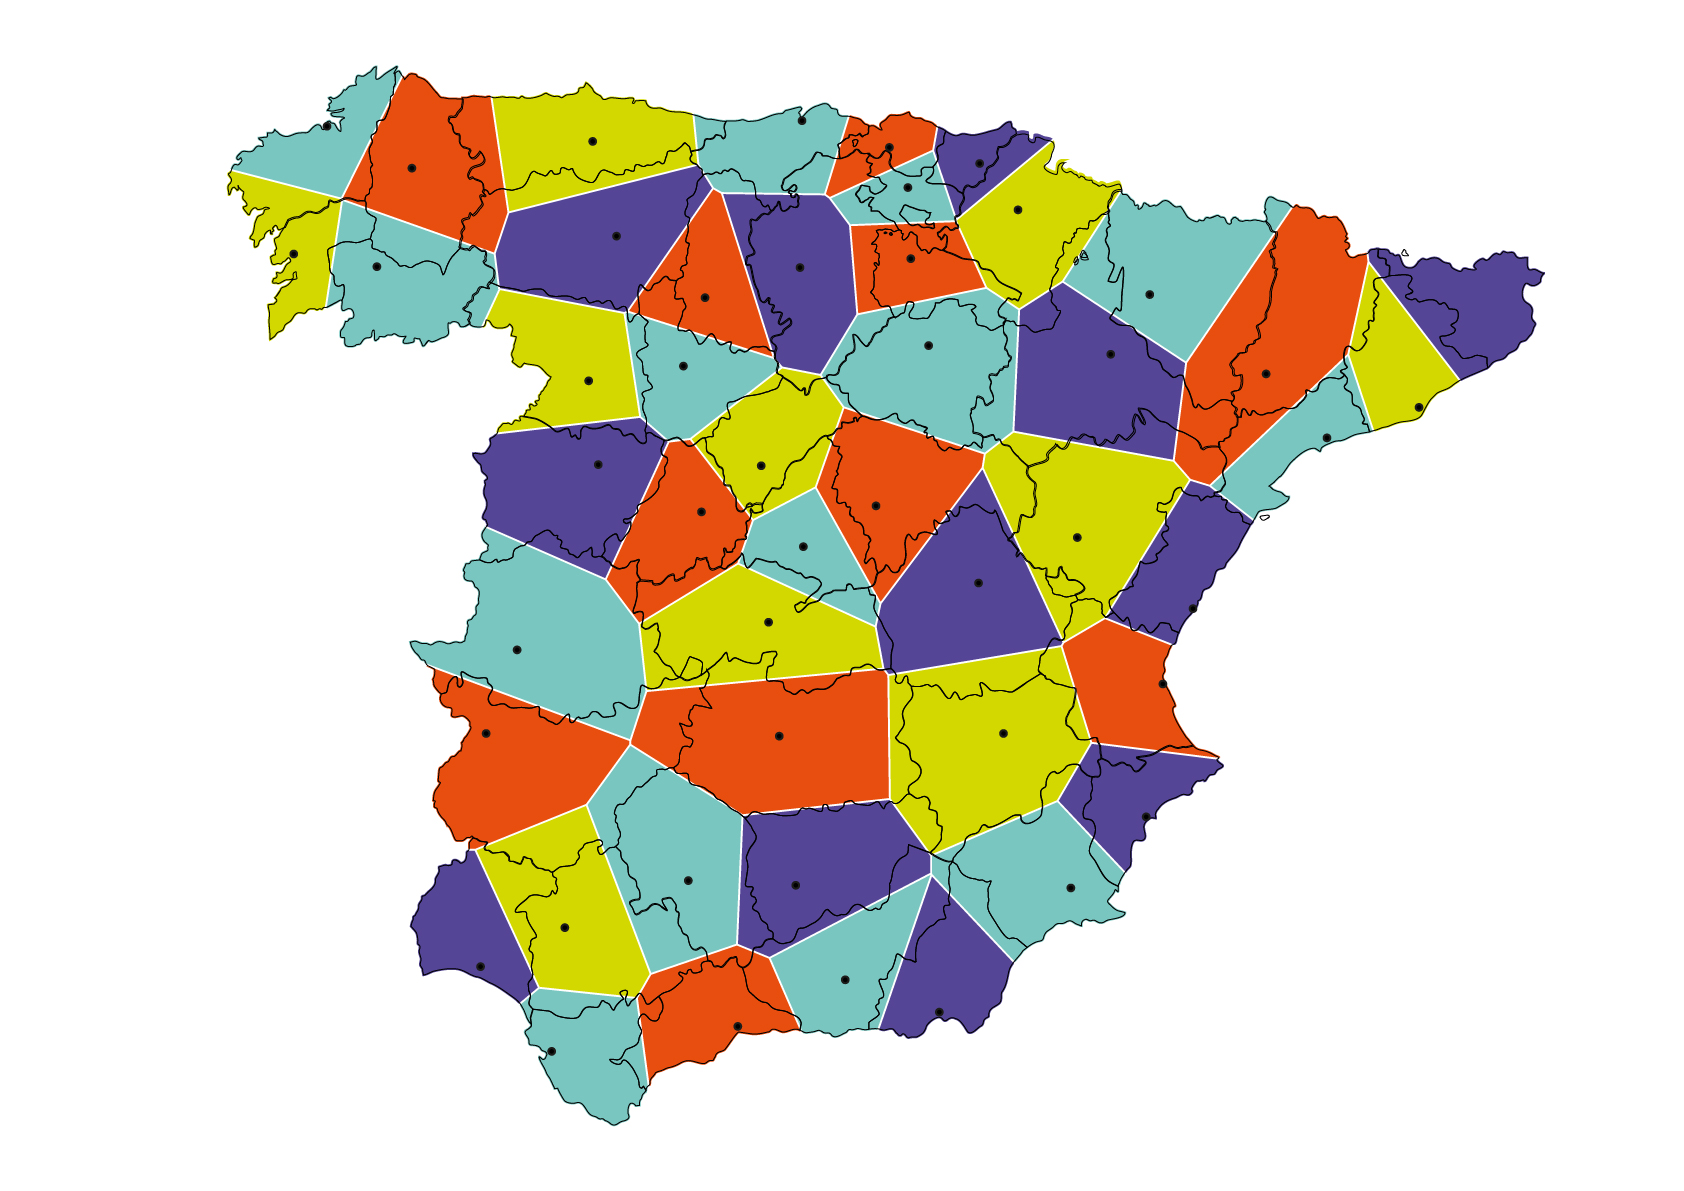
\includegraphics[width=0.60\textwidth]{Imagenes/analisis/voronoi.jpg}
        \caption{Polígonos de Voronoi España} \label{fig:voronoi}
    \end{figure}

    La figura \ref{fig:voronoi} muestra los polígonos de Voronoi obtenido mediante interpolación con método \textit{Nearest Neighbor} de las capitales de provincia de España.
    Este método es empleado en Geomárketing para conocer posibles áreas de influencia, o para realizar regionalizaciones o divisiones territoriales proporcionales.

    \item Vecino natural \\
    La Interpolación de vecinos naturales o \textit{Natural Neighbor}, al igual que la del vecino más cercano, genera polígonos de Voronoi, pero en este caso no se limita a su generación,
    sino que los emplea para realizar ponderaciones a los vecinos más cercanos. 
    
    \begin{figure}[H]
        \centering
        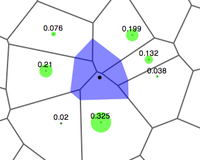
\includegraphics[width=0.30\textwidth]{Imagenes/analisis/vecino-natural.png}
        \caption{Ponderaciones vecinos naturales} \label{fig:vecino-natural}
    \end{figure}

    Una vez generados los polígonos de Voronoi, se crea un nuevo polígono de Voronoi (polígono azul de la figura \ref{fig:vecino-natural}) alrededor del punto desconocido.
    La proporción de superposición entre el polígono azul y los polígonos iniciales se utiliza como ponderaciones.

    \item Distancia Inversa Ponderada \\
    La Distancia Inversa Ponderada o \textit{Inverse Distance Weighted} (IDW), es un método de interpolación que estima los valores desconocidos mediante
    una combinación ponderada de un conjunto de puntos de muestra que se encuentran en su vecindad.
    La influencia de cada punto de la muestra respecto al punto desconocido disminuye con la distancia a este.
    Un ejemplo de uso es la creación de mapas de elevación, como la figura \ref{fig:mapaElev} que vimos en la sección \ref{sec:datos}.
    En este caso el valor desconocido será la elevación y para calcularla se empleará la siguiente función:

    \begin{equation}
        \widehat{z}(x_{j}) = \frac{\displaystyle \sum_{i=1}^{n} \frac{z(x_{i})}{d_{ij}^{p}}}{\displaystyle \sum_{i=1}^{n} \frac{1}{d_{ij}^{p}}} \nonumber
    \end{equation}

    En donde los valores de elevación \textit{z} de los \textit{n} puntos muestrales $x_{i}$ utilizados en la estimación, con respecto a la distancia $d_{ij}$ al punto desconocido $x_{j}$, se agregan mediante un sumatorio.
    La suma de la distancia inversa, que aparece en el denominador, sirve para normalizar el resultado de elevación del punto desconocido, 
    es decir, para que tome valores de elevación comprendidos entre el mínimo y el máximo de los valores de elevación conocidos.
    El parámetro \textit{p}, corresponde a la elevación a una potencia matemática que permite controlar la influencia de los puntos conocidos respecto al punto desconocido.
    Para valores altos de \textit{p}, los puntos más cercanos tienen mayor influencia, de modo que la superficie resultante será menos suave, teniendo mayor detalle.
    Para valores más bajo, los puntos circundantes adquirirán más influencia que los que están más lejos, lo que resulta en una superficie más suave.
    El valor predeterminado de \textit{p} es 2 y un valor superior a 30 deja de tener uso aplicativo.

    \begin{figure}[H]
        \centering
        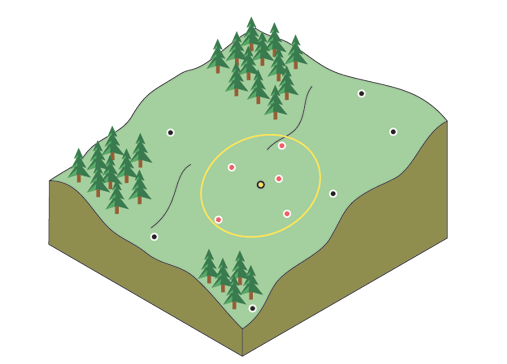
\includegraphics[width=0.60\textwidth]{Imagenes/analisis/IDW.png}
        \caption{Distancia Inversa Ponderada en mapa de elevación} \label{fig:idw}
    \end{figure}

    También se puede limitar los puntos interpolados, especificando un radio alrededor del punto desconocido, de modo que utilicemos los puntos de la muestra que se encuentren en el interior de este.
    En la figura \ref{fig:idw} vemos que aunque tengamos un conjunto de puntos de muestra (puntos rojos y azules), sólo se emplean los puntos más próximos (puntos rojos) para realizar la interpolación.
    El radio de búsqueda puede ser fijo o variable.
    En caso de ser fijo, se deberá establecer un número mínimo de puntos, de modo que si hay menos puntos dentro del radio, este aumentará hasta llegar al mínimo de puntos estipulado.
    En los radios de búsqueda variables, se establecer un número de puntos, lo que provoca que la distancia del radio varíe en función de la densidad de los puntos conocidos cercanos al punto desconocido. 
    En este caso, se puede especificar una distancia máxima del radio de búsqueda. 
    Taambién existe la posibilidad de añadir barreras que limitan la búsqueda de los puntos de muestra, impidiendo seleccionar los puntos que se encuentran detrás de ellas.
    Estas barreras se añaden en forma de polilíneas sobre la superficie que se analiza y pueden representar barreras de ruido, acantilados, carreteras, entre otros.
    
    \item Red Irregular Triangulada \\
    La Red Irregular Triangulada o \textit{Triangulated Irregular Network} (TIN), es una representación vectorial de la superficie formando una malla triángulos no superpuestos, 
    cuyos vértices se calculan a partir de son los puntos muestrales de valores conocidos.

    \begin{figure}[H]
        \centering
        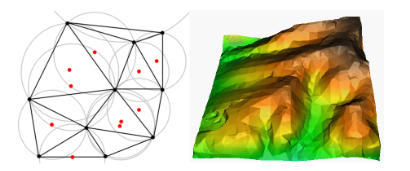
\includegraphics[width=0.60\textwidth]{Imagenes/analisis/TIN.png}
        \caption{Triangulación de Delaunay} \label{fig:tin}
    \end{figure}

    El algoritmo TIN para generar esa malla de triángulos más empleado es la triangulación de Delaunay, 
    en la que se crea circunferencias alrededor de los puntos de muestra, conectando algunas de sus intersecciones, de modo que la circunferencia que da lugar a de cada triángulo de la red no debe contener ningún vértice de otro triángulo. 
    Esto lo podemos ver mejor en la representación de la figura \ref{fig:tin}, en donde también podemos ver el superficie TIN interpolada resultante
    
    Las aristas de las TIN pueden representar la posición de entidades lineales que desempeñan un papel importante en la superficie, como una cresta montañosa o un río.
    Cada triángulo representa una zona homogénea en la que la variable espacial toma valores semejantes. 
    Destaca su uso en la representación de modelos digitales de elevación, aunque puede aplicarse en otros campos, por ejemplo empleando variables ambientales.
\end{itemize}

\section{Otras técnicas de análisis espacial vectorial}

\subsection{Zonas buffer o de influencia}

Las zonas buffer o zonas de influencia son polígonos que envuelven objetos vectoriales con una distancia especificada.
Según el CRS empleado, tenemos varias formas de medir las distancias, dando lugar a zonas buffer euclidianas y geodésicas.
Las zonas buffer euclidianas se crean cuando los objetos de entrada tienen un Sistema de Coordenadas Proyectadas y las geodésicas en los casos de emplear un Sistema de Coordenadas Geográficas.
En ambos casos el valor de la distancia tiene que estar en unidades métricas, por defecto en metros.

\begin{figure}[H]
    \centering
    \subfigure[Puntos]{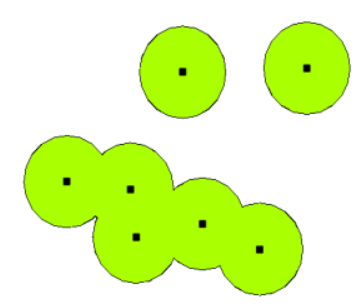
\includegraphics[width=0.20\columnwidth]{Imagenes/analisis/buffer-punto.png}}
    \subfigure[Polilíneas]{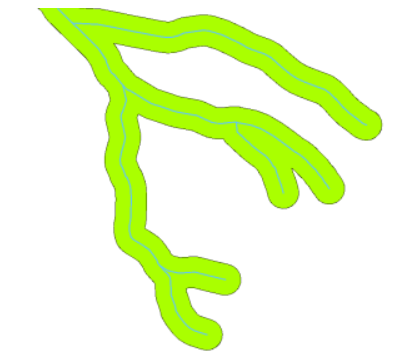
\includegraphics[width=0.20\columnwidth]{Imagenes/analisis/buffer-linea.png}}
    \subfigure[Polígonos]{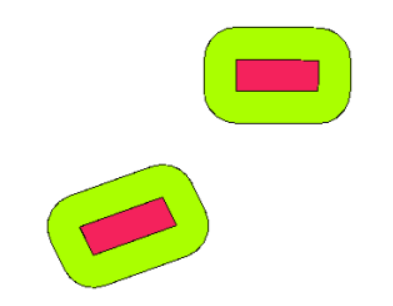
\includegraphics[width=0.20\columnwidth]{Imagenes/analisis/buffer-poligono.png}}
    \caption{Zonas buffer alrededor de objetos vectoriales} \label{fig:buffer} 
\end{figure} 

En la figura \label{ref:buffer} vemos zonas buffer generadas a partir de puntos, polilíneas y polígonos. 
El tamaño de la zona buffer puede variar en función de atributos de los datos espaciales incluidos en la capa vectorial.
Por ejemplo, el ancho de una zona buffer a lo largo de la ribera de un río puede variar dependiendo del de uso de los terrenos adyacentes.
Otra cosa que podemos haces es configurar las zonas buffer alrededor de polilíneas, ríos o carreteras, para que se generen sólo a un lado de la línea.
En estos casos, el lado se elige en función de la dirección desde el punto de inicio hasta el punto final de la linea definida durante su digitalización.
 
Las zonas buffer se utilizan a menudo para proteger el medio ambiente, proteger zonas residenciales o comerciales de accidentes industriales o desastres naturales, o para prevenir la violencia.
Algunos tipos habituales de zonas buffer pueden ser los cinturones verdes entre zonas residenciales y comerciales, zonas fronterizas entre países, 
zonas de protección acústica alrededor de aeropuertos, o zonas de protección de la contaminación a lo largo de los ríos, etc.

\subsection{Superposición espacial}
Superposición espacial es un proceso que permite identificar las relaciones entre dos entidades poligonales que comparten todo o parte de la misma superficie. 
El vector de salida es una combinación de la información de las entidades de entrada.
En términos de GIS, la superposición espacial se realiza sobre dos capas vectoriales (capas de entrada) y da como resultado otra capa vectorial (capa de salida). 

Vamos a emplear las siguientes capas de entrada:
\begin{figure}[H]
    \centering
    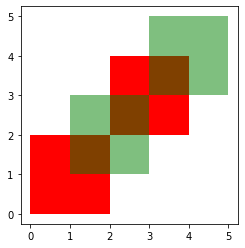
\includegraphics[width=0.30\textwidth]{Imagenes/analisis/capas-superposicion.png}
    \label{fig:capas-superposicion}
\end{figure}
Vemos dos capas, una de color verde y otra de color rojo, formadas por dos cuadrados cada una del mismo tamaño.

\begin{figure}[H]
    \centering
    \subfigure[Intersección]{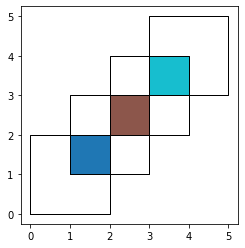
\includegraphics[width=0.33\columnwidth]{Imagenes/analisis/interseccion.png}\label{fig:interseccion} }
    \subfigure[Unión]{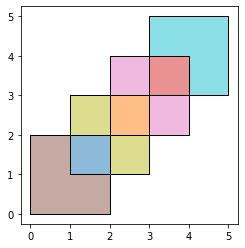
\includegraphics[width=0.33\columnwidth]{Imagenes/analisis/union.png}}
    \subfigure[Diferencia simétrica]{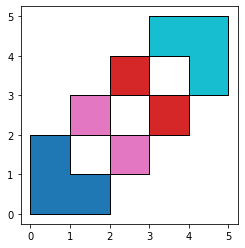
\includegraphics[width=0.33\columnwidth]{Imagenes/analisis/diferencia-simetrica.png}}
    \subfigure[Diferencia]{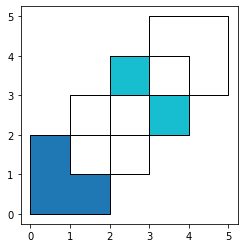
\includegraphics[width=0.33\columnwidth]{Imagenes/analisis/diferencia.png}}  
    \caption{Tipos de superposición espacial} \label{fig:superposicion} 
  \end{figure} 
  
La figura \ref{fig:superposicion} muestra los ejemplos típicos de superposición espacial.

\begin{itemize}
    \item Intersección: La capa de salida contiene las áreas donde las capas de entrada se solapan.
    \item Unión: La capa de salida contiene una combinación de las áreas de las capas de entrada.
    \item Diferencia simétrica: La capa de salida contiene todas las áreas de las capas de entrada excepto aquellas áreas en donde las capas se intersectan.
    \item Diferencia: La capa de salida contiene todas las áreas de la primera capa de entrada (color rojo) que no intersectan con la segunda capa de entrada (color verde).
\end{itemize}

